\chapter{Computational Study}\label{chap:comp}

This chapter presents our computational study and is structured as follows: 
Section \ref{sec:data} describes the data our experiments are conducted on.
Section \ref{sec:samplesize} examines how different samples sizes used for training affect the test error.
In Section \ref{sec:hpo}, we optimize model hyperparameters and seek to get better intuition for parameter configuration by analyzing parameters that are considered for the optimization.
Last but not least, section \ref{sec:noise} demonstrates how noise affects predictive performance of our models.

\section{Data Exploration}\label{sec:data}
The available data set is provided by \cite{Hildebrandt2020_EAT} who create a dataset using the RMDP instances originally used in \cite{UlmerRMDP}. It comprises 850.469 samples with 23.341 unique customer locations, a delivery fleet of 15 vehicles and 15 unique restaurant locations. 

The temporal and spatial distribution of the orders is depicted in figure \ref{fig:dists}. 
Panel (a) of figure \ref{fig:dists} shows the order behaviour of customers. The x-axis denotes the day time in minutes, the y-axis denotes the relative frequency of incoming customer orders for a given day time on the y-axis. We can observe that the order time behaviour across all customers follows a bimodal gaussian distribution. The order frequency peaks at around 12:00 a.m (roughly 700 minutes of day time) and again around 6.00 p.m (roughly 1100 minutes of day time). This indicates that the probability of an order taking place during lunch or dinner time is relatively high.  
Panel (b) of figure \ref{fig:dists} shows the spatial distribution of customer and restaurant locations. The x- and y-axis show the location longitudes and the latitudes respectively. The blue points represent customers, the orange points depict the restaurant locations. There we can see that the majority of restaurants is located where the density of customer locations is rather high. 
\begin{figure}[h]
	\centering
	\subfigure[Request arrival time distribution]{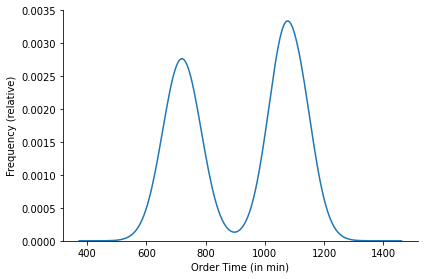
\includegraphics[width=0.49\linewidth]{../Implementation/DataDescription/order_time_dist.png}}
	\subfigure[Spatial distributions]{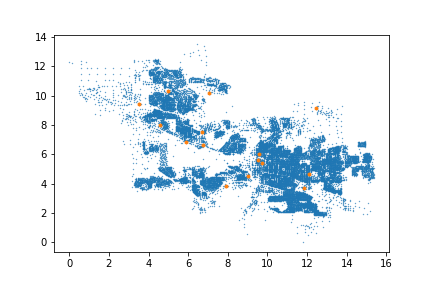
\includegraphics[width=0.49\linewidth]{../Implementation/DataDescription/spatial_dist.png}}
	\caption{Spatial and Temporal Distributions}
	\label{fig:dists}
\end{figure}

Panel (a) of figure \ref{fig:prepdelay} shows the distribution of delivery delay times in minutes for all requests in the data. The delivery delay is here defined as the difference between actual and the expected time of arrival based on PoM. First, we observe that roughly 14-15\% of the requests in our data are delivered on time. Negative values for the delivery delay on the plot indicate that a rather tiny amount of orders happens to be delivered earlier than expected. However, we are most interested in the orders that are actually delivered later than expected. We observe that a non-trivial amount of orders is delivered with a delay of up to 20 minutes. The MSE for predictions based on PoM is approximately 58.0777. As our results will show, arrival time estimation via supervised learning is a vastly better option compared to planning on means.
Since arrival times are impacted by uncertainty in meal preparation times, we take a look at their distribution in our data as well. In panel (b) of figure \ref{fig:prepdelay}, we observe that roughly a fifth of the orders had a preparation time of around 10 minutes. However, a non-trivial amount of orders seem to have quite longer preparation times ranging from 15 to less than 40 minutes. 
\begin{figure}[h]
	\centering
	\subfigure[Delivery delay distribution]{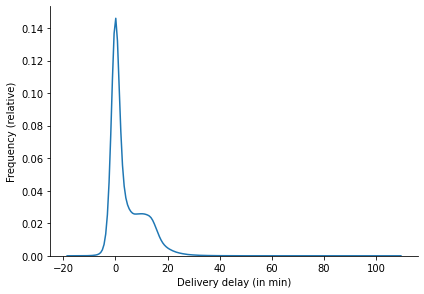
\includegraphics[width=0.49\linewidth]{../Implementation/DataDescription/delivery_delay.png}}
	\subfigure[Meal preparation time distribution]{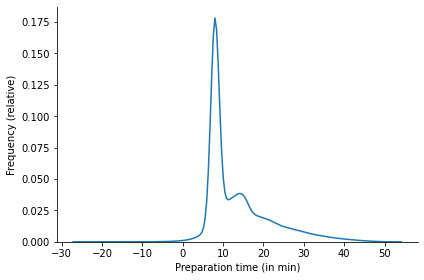
\includegraphics[width=0.49\linewidth]{../Implementation/DataDescription/prep_time.png}}
	\caption{Delivery Delay and Preparation Time Distribution}
	\label{fig:prepdelay}
\end{figure}

\section{Experiment: Sufficient Sample Sizes}\label{sec:samplesize}

This section compares how a difference in sample size impacts the test error for each possible combination of our models and datasets. Since less samples in the training data correspond to lower training times, we use the results of this experiment for the subsequent time consuming hyperparameter optimization to speed our experimental procedure up. For our linear model and the considered ensembles, we consider 100 training runs with every run corresponding to a sample subset of size $ \{2000, 4000, \dots,\\ 200.000\} $. For each model, we set the parameters manually found by trial-and-error since we did not conduct the hyperparameter optimization yet. For GBDT, we set the learning rate to 0.02, the number of estimators to 1000 and enable early stopping with a patience of 20. For Random Forest, we set the number of estimators again to 1000 and subsample 80\% of the samples from only 80\% of the features in every iteration. For Random Forest, we enable early stopping with a patience of 20 as well. Every run of every test instance is validated on the same independent validation set which contains 20\% of our total amount of samples. 

Figure \ref{fig:convergences} shows the model performances on both datasets with increasing sample sizes. In all panels, the x-axis depicts the sample size in a training run, and the y-axis represents the mean squared test error (MSE) of that run. GBDT, Random Forest and Linear Regression belong to their own panels (a), (b), and (c) respectively. For GBDT and Random Forest, we observe that a sample size of 200.000 seems to be sufficient since the models, whether they are trained on the raw or the crafted data, begin to converge there. For GBDT, the MSE at a sample size of 200.000 is approximately 26 when trained on the raw data, and between 27-28 when trained on crafted data. Random Forest performs slightly worse on both datasets when compared to GBDT. However, when less are used for training, in contrast to GBDT and Random Forest, the linear model has a poorer performance on both datasets with a MSE that converges around slightly more than 30 on the raw set and roughly at a little bit more than 31 on the crafted set. However, the linear model converges almost immediately when trained on the crafted dataset while slightly less than 25.000 samples are needed in order for the linear model to converge when we train it on the raw dataset. Surprisingly, we observe a sudden spike of the test error close to the very beginning for the linear model when trained on the raw data. Moreover, there is only a marginal difference between the performances of the linear model on the different datasets which is not the case for GBDT and Random Forest.
All in all, we conclude the following:
\begin{description}[font=$\bullet$\scshape\bfseries]
	\item All models perform consistently better when trained on the raw dataset
	\item GBDT returns the best results for both datasets
	\item Regardless of the datasets, the linear model needs the least samples in order to converge. However, GBDT and Random Forest significantly outperform the linear model consistently. 
\end{description}
\begin{figure}[h]
	\centering
	\subfigure[For GBDT]{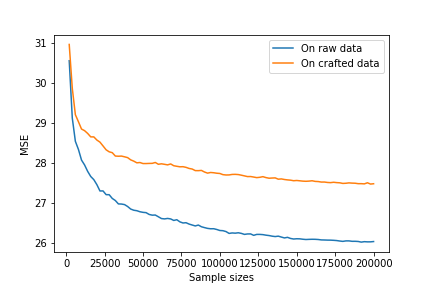
\includegraphics[width=0.49\linewidth]{../Implementation/SampleSize/GBDT_SampleSizes.png}}
	\subfigure[For Random Forest]{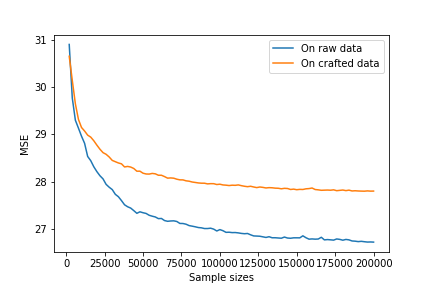
\includegraphics[width=0.49\linewidth]{../Implementation/SampleSize/RF_SampleSizes.png}}
	\subfigure[For Linear Regression]{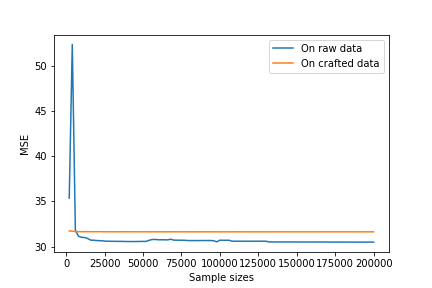
\includegraphics[width=0.49\linewidth]{../Implementation/SampleSize/LR_SampleSizes.png}}
	\caption{MSE for Different Sample Sizes}
	\label{fig:convergences}
\end{figure}

\section{Experiment: Hyperparameter Analysis}\label{sec:hpo}
This section presents the hyperparameter optimization (HPO) experiments conducted for GBDT and Random Forest. 
We use \textit{Optuna}, a popular HPO framework proposed and designed by \cite{akiba2019optuna}, to conduct our HPO experiments. 
\textit{Optuna} provides a simple implementation design that allows us to analyze several parameters of choice from different points of view. 
The optimizations were conducted on both the crafted data set and the raw data set. 
Concretely, we will proceed as follows: First, we will present the hyperparameters we decided to include in the HPO, then present the optimal hyperparameter values resulting from the experiment and explore the predictive power of different parametrizations. 
For every GBDT and RF experiment instance, we will use the \textit{Optuna}-implementation of \textit{CMA-ES} to sample values from the respective search spaces of the parameters considered for optimization. To speed up the optimization process, we use the \textit{Optuna}-implementation of the \textit{Hyperband Pruner} presented in \cite{li2018hyperband}.
We will use the \textit{optuna} implementation of \textit{fANOVA} presented in \cite{fANOVA} to determine hyperparameter importances. 
For each parameter importance prediction, we set the number of estimators in \textit{fANOVA} to 1000.
For both datasets respectively, we will use 200.000 samples for training, and 20\% of all samples as the validation set.
\subsection{GBDT}

In this subsection, we will conduct HPO experiments for GBDT on both datasets. 
Besides the parameters considered for optimization, we set the number of estimators for HPO run to 1000 and enable early stopping with a patience of 20. The selection of the parameter search spaces is the result of trial-and-error since machine learning problems are highly individual and, as we have already demonstrated with our literature review, different solution approaches for quite similar problems are possible. The determination of parameter values and parameter search spaces therefore has to happen at least partly in a manual fashion, which is why we regard the trial-and-error heuristic as a suitable approach for the configuration of hyperparameter values and hyperparameter search spaces for our HPO. Detailed descriptions of the considered parameters for the \textit{lightgbm}-GBDT implementation can be found under \url{https://lightgbm.readthedocs.io/en/latest/Parameters.html}. For GBDT, following parameters and search spaces are considered for optimization:
\begin{description}[font=$\bullet$\scshape\bfseries]
	\item $ \text{learning\_rate} \in [0.01, 0.05] $ in steps of 0.001.
	\item $ \text{max\_depth} \in [5, 100] $ in steps of 0.001.
	\item $ \text{feature\_fraction} \in [0.1, 1.0] $ in steps of 0.01.
	\item $ \text{feature\_fraction\_bynode} \in [0.3, 1.0] $ in steps of 0.01
	\item $ \text{num\_leaves} \in [20, 300] $ in steps of 1
	\item $ \text{min\_child\_samples} \in [10, 400] $ in steps of 1.
	\item $ \text{subsample\_freq} \in [1, 10] $ in steps of 1.
	\item $ \text{subsample} \in [0.3, 1.0] $ in steps of 0.01.
\end{description}

The exact optimal parameter configurations for GBDT on both datasets is depicted in figure \ref{fig:GBDT_Optimal}. Training GBDT with the respective optimal parameter configuration using the full available amount of samples with 20\% of it as our validation set results in a mean squared error of approximately 25.1384 on the raw data, and 27.0852 on the crafted data. Early Stopping does not set in when training GBDT on raw data, whereas it does set in for the crafted data at around 600. 
\begin{figure}[h]
	\centering
	\subfigure[Optimal Configurations]{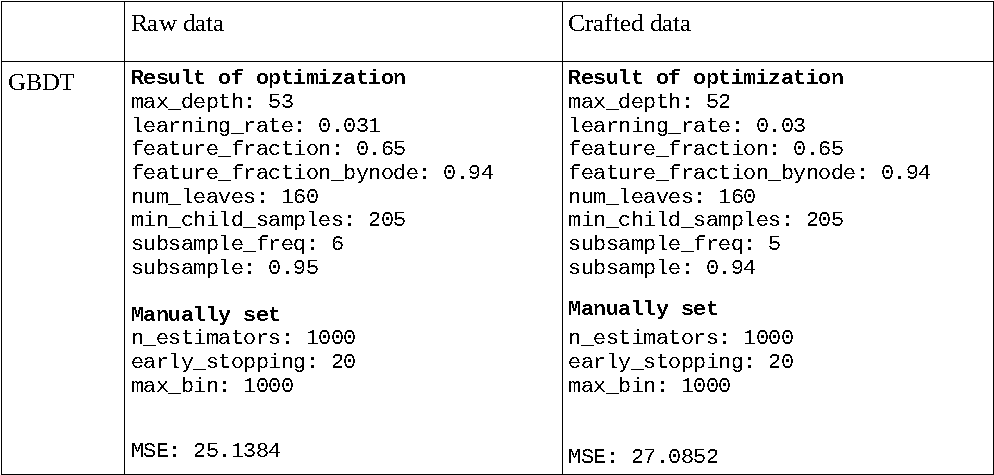
\includegraphics[width=\linewidth]{figures/HPO/GBDT_ResultsTable_HPO_Optimal.pdf}}
	\subfigure[Training History on Raw Data]{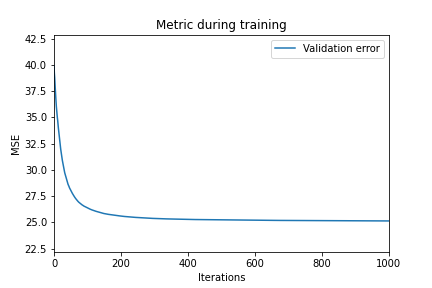
\includegraphics[width=0.49\linewidth]{../Implementation/optunaStudies/GBDT_Raw_Optim_Metric.png}}
	\subfigure[Training History on Crafted Data]{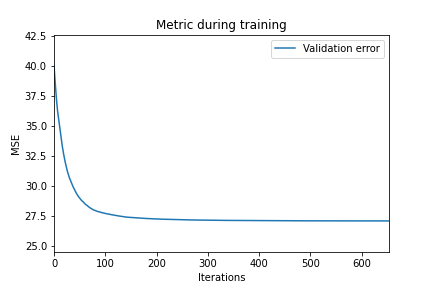
\includegraphics[width=0.49\linewidth]{../Implementation/optunaStudies/GBDT_Crafted_Optim_Metric.png}}
	\caption{Optimal Configurations and Training Histories for GBDT}
	\label{fig:GBDT_Optimal}
\end{figure}

Figure \ref{fig:GBDT_ParallelPlot} depicts the parameter configurations of each optimization epoch in form of a parallel coordinate plot for GBDT on raw data in panel (a) and on crafted data in panel (b). Except the vertical gray line at the very left in the plots, each vertical gray axis represents the values ranging within the defined intervall of its corresponding parameter, whereas the very left line represents the axis for the objective values. The lines connecting all the parameter axes represent the parameter configurations of the optimization epochs. The bluer a line, the better the objective value - in our case the mean squared error. 
At first glance, it can be seen directly that the parameter configurations of both plots for good predictive performance are quite similar. For both sets, the mean squared error is minimized when we roughly use two-thirds of the features for each GBDT iteration (feature\_fraction, feature\_fraction\_bynode). Less test error is more likely achieved when we allow the algorithm to build rather deep trees up to a maximal depth of 50 while constraining the tree splitting process by specifying a lower bound of around 200 for the minimal amount of samples a node must contain in order to split it further (min\_child\_samples). We can furthermore see that a better objective value is attained when using nearly all samples considered for a GBDT iteration rather than applying (subsampling) and learning rates ranging between 0.03 to 0.05 (learning\_rate).

\begin{figure}[h]
	\centering
	\subfigure[On raw data]{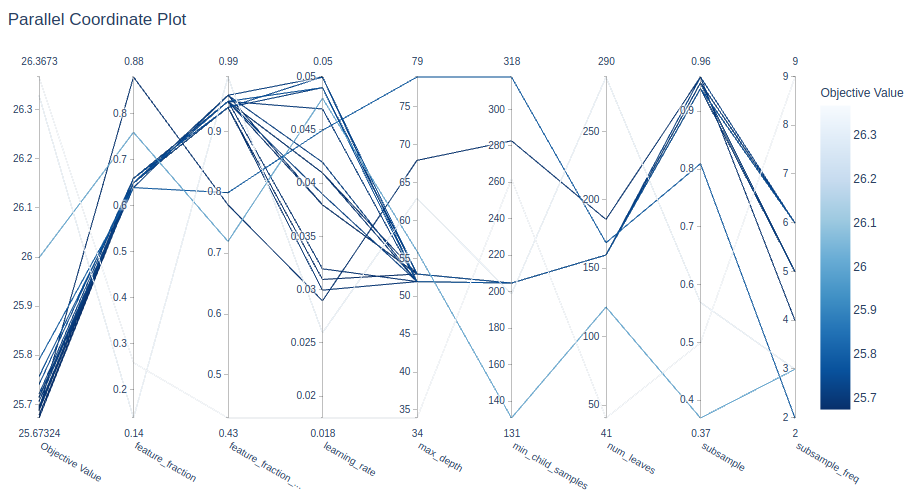
\includegraphics[width=\linewidth]{figures/HPO/GBDT_HPO_Raw_ParallelPlot.png}}
	\subfigure[On crafted data]{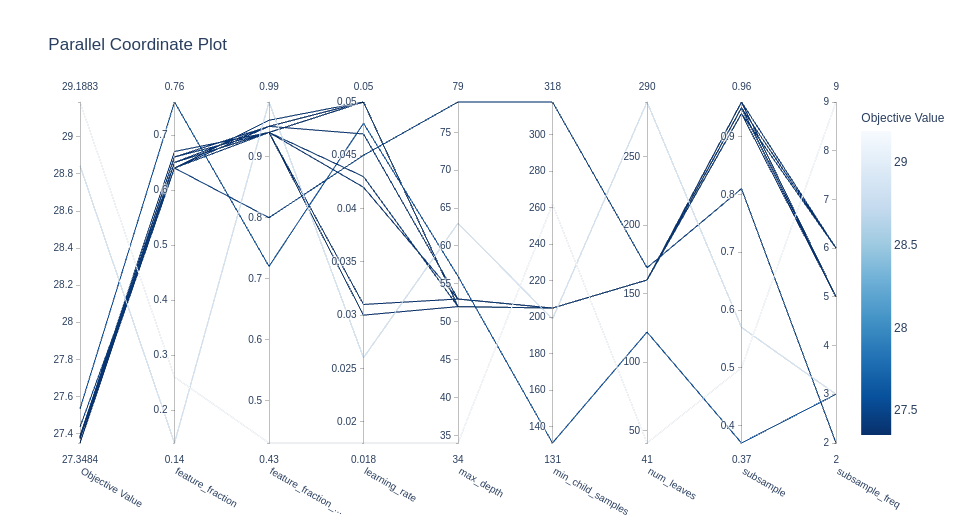
\includegraphics[width=\linewidth]{figures/HPO/GBDT_HPO_Crafted_ParallelPlot.png}}
	\caption{Parallel Coordinate Plots for GBDT}
	\label{fig:GBDT_ParallelPlot}
\end{figure}

Up next are the hyperparameter importances of GBDT depicted in figure \ref{fig:GBDT_Importances}. Panel (a) shows the importances for GBDT when trained on raw data
Panel (b) shows the importances for GBDT when trained on crafted data.
The x-axis of the importance plots depicts the relative parameter importances. 
The y-axis is categorical and shows the parameters we consider to optimize. 
We can observe that the results for the datasets GBDT was trained on differ significantly. 
For GBDT on the raw data, we observe that choosing the right amount for subsampling, a suitable learning rate for calculating the gradient in GBDT, and the right feature fraction are of highest importance. For GBDT on the crafted data, we observe that the learning rate and the feature fraction are of even more relative importance, whereas the parameter for subsampling has far less significant impact on the objective value as compared to GBDT on raw data. 
We further observe non-trivial differences in relative importance for the subsampling frequency showing a difference 7\%, and for \textit{min\_child\_samples} with a difference of 5\%. For both datasets, the number of leaves, the percentage of features fractioned per node, and the maximal depth constraint for the estimators remain nearly equally important.   
\begin{figure}[h]
	\centering
	\subfigure[On raw data]{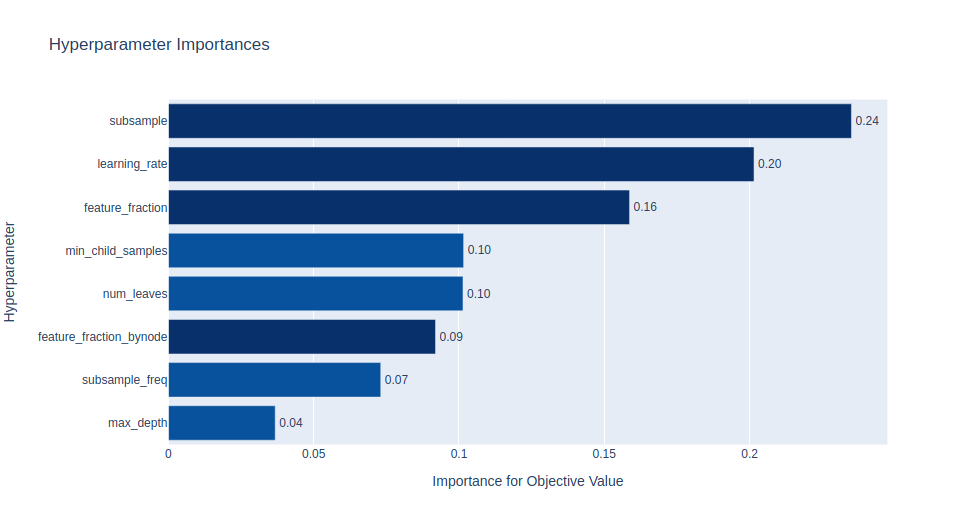
\includegraphics[width=\linewidth]{figures/HPO/GBDT_HPO_Raw_Importances.png}}
	\subfigure[On crafted data]{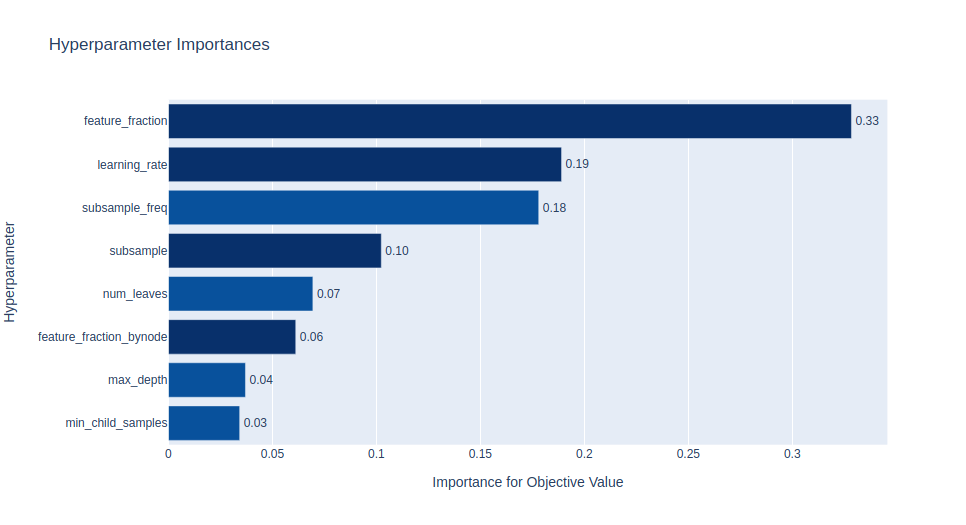
\includegraphics[width=\linewidth]{figures/HPO/GBDT_HPO_Crafted_Importances.png}}
	\caption{Hyperparameter Importances for GBDT}
	\label{fig:GBDT_Importances}
\end{figure}

We conclude the following: 
\begin{description}[font=$\bullet$\scshape\bfseries]
	\item Although there are significant differences between the hyperparameter importances for both GBDT experiment instances, the resulting optimal configuration of both does hardly differ. Thereby, we suggest that the difference in relative parameter importances does not affect the outcome of the optimization. We also suggest that the importances depend on the features that are used.
	\item GBDT consistently performs better when trained on the raw data model. This could be due to the reason that, besides the features both sets have in common, our raw set includes exact routing information of every action on the customer's route, whereas the crafted set in contrast includes only the stop features.
\end{description}
\clearpage
\subsection{Random Forest}
In this subsection, we will conduct HPO experiments for Random Forest on both datasets. 
For Random Forest, we decided to optimize following parameters and set the search spaces for each of them as follows:
\begin{description}[font=$\bullet$\scshape\bfseries]
	\item $ \text{max\_depth} \in [5, 100] $ in steps of 1.
	\item $ \text{feature\_fraction} \in [0.3, 1.0] $ in steps of 0.01.
	\item $ \text{feature\_fraction\_bynode} \in [0.3, 1.0] $ in steps of 0.01
	\item $ \text{num\_leaves} \in [900, 1200] $ in steps of 1
	\item $ \text{subsample\_freq} \in [1, 10] $ in steps of 1.
	\item $ \text{subsample} \in [0.3, 0.99] $ in steps of 0.01.
\end{description}
Besides the parameters considered for optimization, we set the number of estimators for one iteration in Random Forest to 1000 and enable early stopping with a patience of 20 as we did for the GBDT optimization. Additionally, we set \textit{min\_child\_samples} to 1 and thus exclude it from the set of parameters considered for optimization, because by trial-and-error we found that \textit{lightgbm-RF} performs best when it is set very low. For the same reason, we set \textit{min\_data\_in\_bin} to 1. Again, we are going to analyze optimal configurations with the help of the corresponding parallel plots first and then examine the hyperparameter importances for Random Forest trained on each dataset. 

Figure \ref{fig:RF_Optimal} depicts the optimal parameter configurations resulting of the HPO for the considered parameters and the respective training histories. We observe that Random Forest on the raw data returns a lower test error of 26.5538 compared to the crafted features with a test error of 27.7938 when trained on their respective optimal parameter configurations and with the full amount of samples available. Early Stopping sets in at around 170 iterations for the raw data instance, and at roughly 70 for the crafted data experiment instance. 
\begin{figure}[h]
	\centering
	\subfigure[Optimal configurations]{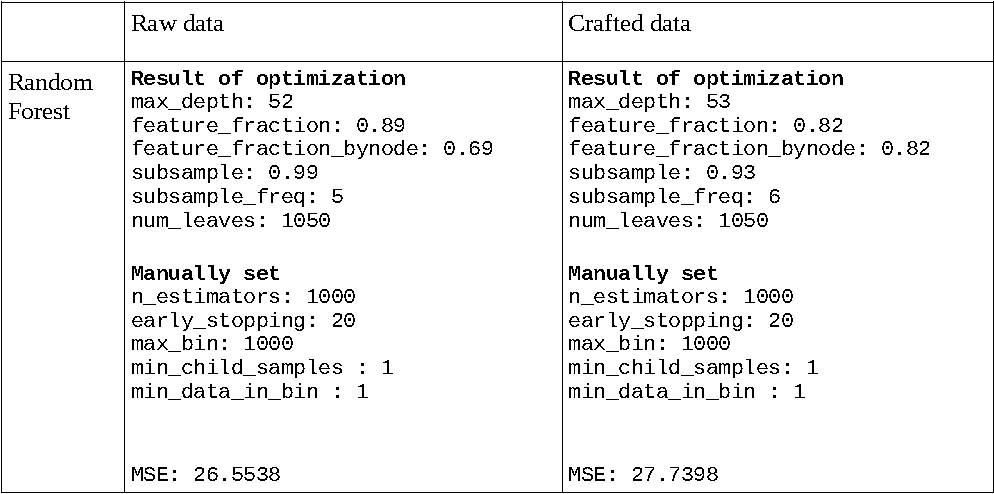
\includegraphics[width=\linewidth]{figures/HPO/RF_ResultsTable_HPO_Optimal.pdf}}
	\subfigure[Training History on Raw Data]{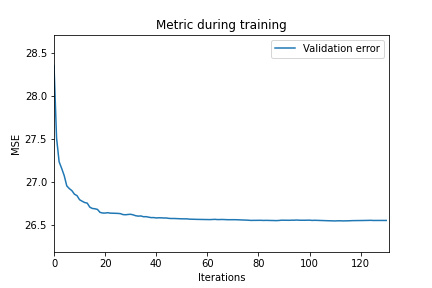
\includegraphics[width=0.49\linewidth]{../Implementation/optunaStudies/RF_Raw_Optim_Metric.png}}
	\subfigure[Training history on Crafted Data]{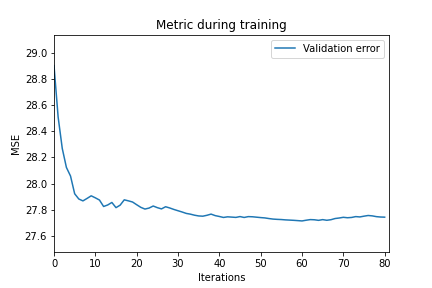
\includegraphics[width=0.49\linewidth]{../Implementation/optunaStudies/RF_Crafted_Optim_Metric.png}}
	\caption{Optimal Configurations and Training Histories for Random Forest}
	\label{fig:RF_Optimal}
\end{figure}

Figure \ref{fig:RF_ParallelPlot} depicts the parallel coordinate plots for Random Forest on the raw and crafted features in panel (a) and (b) respectively. We observe that the distribution of parameter configurations achieving a comparably well objective value is quite similar. A minimized objective value is achieved when the feature fraction and the feature fraction by node used for each estimator range between 0.8 and 1. Furthermore, the maximal depth constraint set at a rather high value ranging between 50 and 60 seems to be optimal according to the HPO. In the majority of optimal cases, the number of leaves each estimator has at the end of the iteration is very high with roughly 1050 leaves. For subsampling, we observe that setting subsampling fraction greater than 90\% in a frequency of 6 is associated with a minimized test error.
\begin{figure}[h]
	\centering
	\subfigure[On raw data]{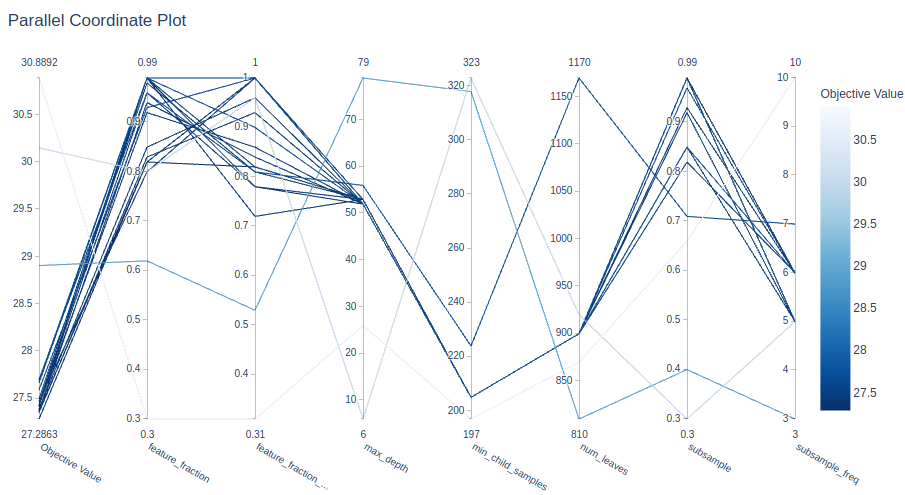
\includegraphics[width=\linewidth]{figures/HPO/RF_HPO_Raw_ParallelPlot.png}}
	\subfigure[On crafted data]{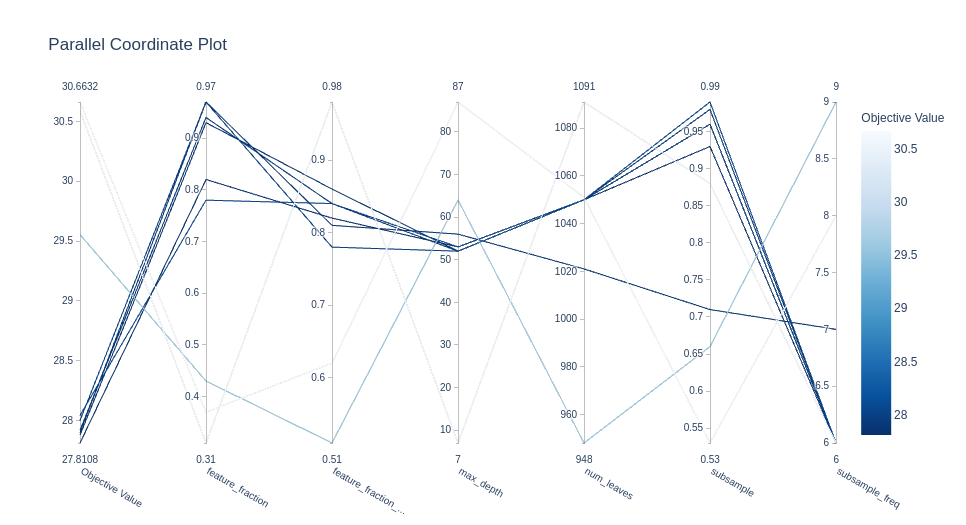
\includegraphics[width=\linewidth]{figures/HPO/RF_HPO_Crafted_ParallelPlot.png}}
	\caption{Parallel Coordinate Plots for Random Forest}
	\label{fig:RF_ParallelPlot}
\end{figure}

The hyperparameter importances for Random Forest on the raw and the crafted data set are depicted in \ref{fig:RF_Importances}. For both instances, we observe that the chosen feature fraction has by far the most impact with a relative importance of 0.43 for the raw data instance, and 0.48 for the crafted data instance. Combining this information with the information given on the parallel plot, we conclude that it is crucial for the performance to set the feature fractions higher than 80\%. The instances significantly differ when it comes to subsampling and the subsampling frequence with differences of 10\% and 11\% respectively. When it comes to the maximum permitted depth and the number of leaves, the instances also show noticeable percentual difference of 6\% and 3\% respectively.
\begin{figure}[h]
	\centering
	\subfigure[On raw data]{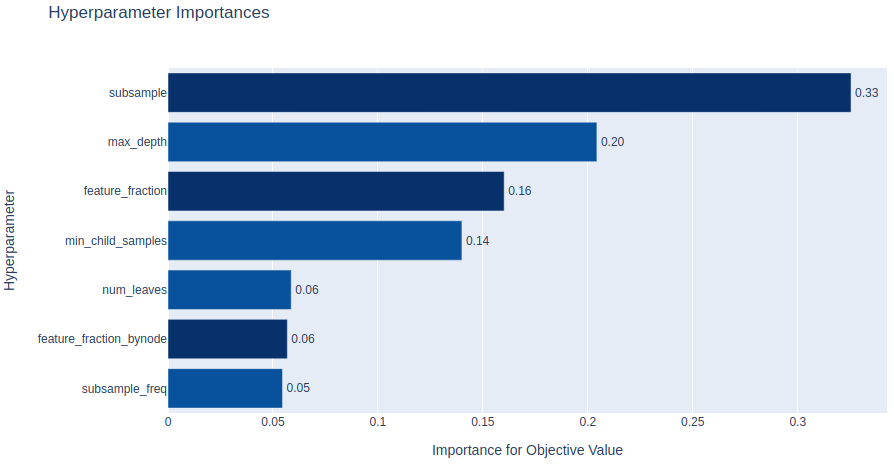
\includegraphics[width=\linewidth]{figures/HPO/RF_HPO_Raw_Importances.png}}
	\subfigure[On crafted data]{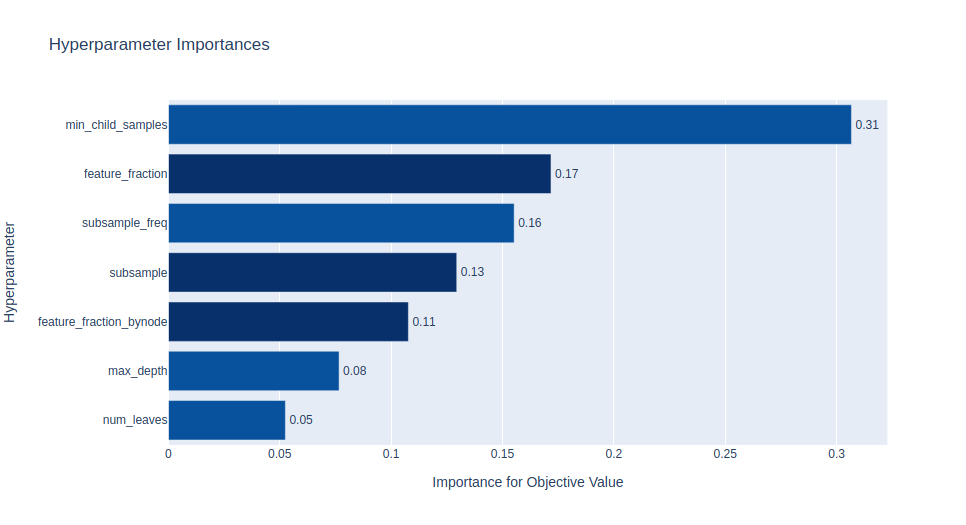
\includegraphics[width=\linewidth]{figures/HPO/RF_HPO_Crafted_Importances.png}}
	\caption{Hyperparameter Importances for Random Forest}
	\label{fig:RF_Importances}
\end{figure} 
We conclude the following:
\begin{description}[font=$\bullet$\scshape\bfseries]
	\item As it was the case for the GBDT instances, the model performs noticeably better when trained on the raw data model.
	\item As it was the case for the GBDT instances, the parameter configurations promising the best results for both Random Forest instances are quite similar while their respective hyperparameter importances do differ. 
	\item We observe that one parameter is impacting the outcome of the model by far the most compared to the other parameters considered for optimization. Such a dominant impact was not observed for the GBDT instances.
\end{description}
\section{Experiment: Noise Induction}\label{sec:noise}
In this experiment, we test the robustness of our models. We do this by randomly sampling values from the Gaussian distribution
\begin{equation}
	p(x) = \dfrac{1}{\sqrt{2\pi\sigma^{2}}} e^{-\dfrac{(x-\mu)^2}{2\sigma^2}}
\end{equation}
with a mean $ \mu $ of 1 and standard deviations $ \sigma \in \Sigma $ in the set of $ \{0.1, 0.2, \dots, 1.0\} $ and adding the resulting value, which is the noise, to the order time, the meal preparation time and the PoM-based expected time of arrival. A higher standard deviation is understood as a wider spread of the distribution, and vice versa. We split the data into training and validation sets with a size of 80\% respectively 20\%. The noise is only added to the training set.

The GBDTs and Random Forests were trained with the optimal parameter configurations resulting from the HPO and on the full size of available samples. Figure \ref{fig:noise} depicts the model performances for different levels of noise on both datasets. Panel (a) shows the GBDT instances, panel (b) the Random Forest instances, and panel (c) and (d) show the results for linear regression. We decided to plot the performances of linear regression separately for both datasets for visualization purposes since the y-axis is scaled vastly different. The x-axis represents the standard deviation, the y-axis shows the mean squared test error.

At first glance, we observe that a higher test error is associated with higher levels of noise for every test instance. GBDT and Random Forest trained on the raw data produce the best results. For them, we observe quite similar behaviour for the different datasets: While both start out fairly close to the value attained in figure \ref{fig:GBDT_Optimal} and \ref{fig:RF_Optimal} with a mean squared error of approximately less than 26 and 28 respectively on the raw set, both show a monotonous increase in test error up to approximately 30 for the highest noise level considered. However, we get significantly different results when we train GBDT and Random Forest on the crafted set. For both models, the MSE starts out with a mean squared error around 30, which is noticeably less than the mean squared error achieved with the configurations for the crafted set depicted in \ref{fig:GBDT_Optimal} and \ref{fig:RF_Optimal}, and rise up to slightly more than 36. We thus conclude that the models trained upon the raw set are significantly more robust when noise is induced. Our linear model produced results that are highly interesting: Despite both panels (c) and (d) in figure \ref{fig:noise} visualizing quite similar looking exponential increases, the resulting MSEs for the different noise levels could not be further away from each other. When trained on raw data, linear regression levels off between 30-31 and is therefore the most robust model in our comparison since its variability in results is by far the lowest. When trained on crafted data however, a consideration of linear regression as a prediction model is no longer an option as the MSE skyrockets to 1200 at a noise level of 1.0. We further note that linear regression on the raw data consistently produces better results than GBDT and Random Forest when trained on the crafted data. 
With respect to the robustness of our models, we conclude the following:
\begin{description}[font=$\bullet$\scshape\bfseries]
	\item Whether we use the raw or the crafted data set for training, GBDT and Random Forest produces the best results. On raw data, GBDT is ahead of random forest, whereas both perform nearly equally good when trained on the crafted data set. 
	\item Out of all models, the linear regression model trained on the noisy raw data is the most robust. Surprisingly, the complete opposite is true when we train linear regression on the crafted data. 
\end{description}
\begin{figure}[h]
	\centering
	\subfigure[For GBDT]{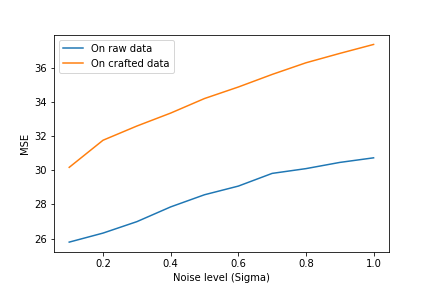
\includegraphics[width=0.49\linewidth]{../Implementation/NoiseStudies/GBDT_Noise.png}}
	\subfigure[For Random Forest]{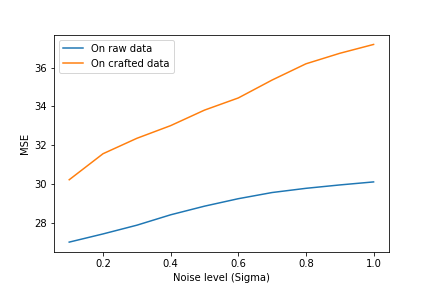
\includegraphics[width=0.49\linewidth]{../Implementation/NoiseStudies/RF_Noise.png}}
	\subfigure[For Linear Regression (Raw)]{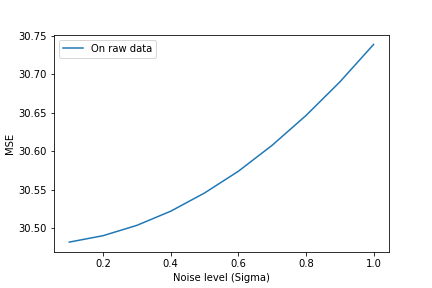
\includegraphics[width=0.49\linewidth]{../Implementation/NoiseStudies/LR_Raw_Noise.png}}
	\subfigure[For Linear Regression (Crafted)]{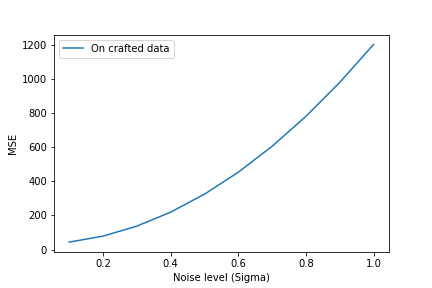
\includegraphics[width=0.49\linewidth]{../Implementation/NoiseStudies/LR_Crafted_Noise.png}}
	\caption{Performance of models for different noise levels on both datasets}
	\label{fig:noise}
\end{figure}



